% !TeX root = ../main.tex

\subsection{Chromatin Coarse-Graining, chromatin as a polymeric fluid}
The coarse-graining procedure performed for this project was inspired by the article written by Kremer and Grest in 1990
\cite{kremerDynamicsEntangledLinear1990a}.

In a very interesting chapter, which is summarized in this section, the book "\textit{Giant molecules: here, there, and everywhere}"
\cite{grosbergGiantMoleculesHere2011}
compares the DNA to a chain of beads, and more in general, to a polymeric fluid inside the cell nucleus. It affirms that the random motion of a DNA fiber could be compared to the stochastic Brownian dynamics of a particle: several small connected segments would move randomly, however maintaining their order and connectivity. It is easy to understand that, given this hypothesis, the most important quantity that should be computed to perform the coarse-graining of a polymer is the length of the rigid segments.

To perform the following steps and derive that value, also called as Kuhn length, it is made the assumption that a DNA polymer moves in a Brownian manner. Although this type of dynamics would largely reduce the volume of the chromatin, still the dimension of the latter would be too high to permit its entire confinement inside the nucleus of any cell. For this reason, it was suggested that some other mechanisms intervene to rule the condensation behavior of the filaments.
\cite{grosbergGiantMoleculesHere2011}. 
For a DNA polymer, the Kuhn length is thought to be approximately equal to 100 nm.

To start, it is defined the difference between a Brownian motion and a straight movement. That discrepancy could be written as follows:

\begin{align*}
    &\text{- For a straight motion } \;\;\;\; R = v(t_2 - t_1) \\ 
    &\text{- For a Brownian particle } \;\;\;\; R = l_{\text{eff}}^{1/2} [v (t_2 - t_1)]^{1/2} 
\end{align*}

Where $R = |\vec{R_1} - \vec{R_2}|$ is the difference between the initial position $\vec{R_1}$ and the final one $\vec{R_2}$. The obtained equation can be rewritten as a square-root displacement in the following way:

$$
    R = l_{\text{eff}}^{1/2} [v (t_2 - t_1)]^{1/2} = \langle(\vec{R_2} - \vec{R_1})^2\rangle^{1/2}
$$

By easily substituting $v (t_2 - t_1)$ with $L$, it is possible to derive the equation for a polymer, which becomes

$$
    R = l_{\text{eff}}^{1/2} * L^{1/2}
$$

Where L is the maximal possible length of the polymer, and is called contour length. By computing the squared value of the previous equation, it is possible to obtain

\begin{align} \label{eq: kuhn length definition}
    & R^2 = l_{\text{eff}} * L = \langle\vec{R}^2\rangle \nonumber\\ 
    & \rightarrow l_{\text{eff}} = \frac{R^2}{L} 
\end{align}

Importantly, the derived equation \ref{eq: kuhn length definition} contains the definition of the Kuhn length $l_{\text{eff}}$. This quantity allows to understand the degree of bendability of the chain. By using a more visual approach, this length could be considered as a memory that is maintained along a path on the polymer. Indeed, keeping in mind the idea of following a "journey" on the chain, the average angle that is obtained at a contour length $s$, obtained through the intersection of the tangents at the starting and the ending points of the segment (figure \ref{fig: journey}), is big or low depending on the ratio between the analyzed and the Kuhn lengths. By looking to the equation \ref{eq: contour length mean angle}, in general, the lower is the contour segment inspected with respect to the Kuhn length, the higher is the probability of having a low degree angle ($\langle\cos{\theta} \sim 1\rangle$). On the contrary, by analyzing larger lengths, it is possible to obtain a wider range of angles, with a calculated cosine that becomes $\langle\cos{\theta} \sim 0\rangle$.

\begin{equation} \label{eq: contour length mean angle}
    \langle \cos{\theta(s)}\rangle = \exp{\left(-\frac{s}{l}\right)}
\end{equation}

\begin{figure}[H] 
    \centering 
    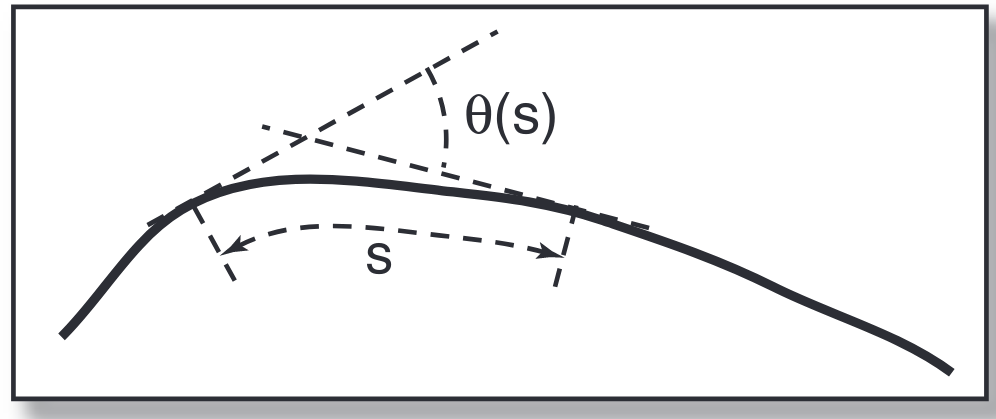
\includegraphics[width=75mm]{persistance_length.png} 
    \caption{Image taken from Grosberg \textit{et al.}\cite{grosbergGiantMoleculesHere2011}. Angle formed between the tangents at the extremes of a contour length.} 
    \label{fig: journey} 
\end{figure}

To conclude, the Kuhn length is directly related the persistance length, which is another quantity, exploited in the polymer model of this work to compute the angle bending potentials, which are calculated through the equation \ref{eq: angle bending potential}. For this project, the relationship between the persistance and the Kuhn lengths was parametrized as in the formula \ref{eq: persistence length}.\\

Because of the fact that it is not really clear which and how many stages of compaction exist (chapter \ref{intro: chromatin}), it was decided to generate chains with beads including 5000 bp. The parameters for the most coarse-grained model (CG) were partially obtained by taking into account a Fine Scale (FS) configuration.

% The Young's modulus ($E$) of a chain is the extent to which a solid material (or a polymeric fluid, in this case) can be deformed
% As Robert Hook noticed, the following is valid 
% \begin{equation}
    %     \sigma = E \frac{\Delta l}{l}
% \end{equation}
% Where $l$ represents the length of the chain and $\Delta l$ the deformation $\sigma$
% \cite{grosbergGiantMoleculesHere2011}

% The entanglement length ($N_e$) corresponds to the Young's modulus that is experimentally found in the plateau region where a force starts to produce irreversible deformations in a chain.

% % #TODO put a reference image if you want


% It is also defined as the "the average number of monomer units along the chain between two nearest effective cross-links."
% and is related to the ability of chains to form knots between each other
% \cite{grosbergGiantMoleculesHere2011}
.

%#TODO add subchapter rosettes
%#TODO about the reason of coarse graining with such a low resolution
%#TODO fine scale e coarse grained model, explain reasons
